\let\textcircled=\pgftextcircled
% \section{Approach and Development Methodology}
% To tackle the challenges of taxpayer verification and compliance scoring, we adopted a structured approach that combines analysis of key indicators and system design. Our process focuses on clearly defining involved entities, identify risk-related factors and defining scoring mechanisms. \\

% For the implementation phase,  we applied the Scrum framework, a lightweight agile method suited for managing complex product development. Scrum promotes incremental development through short, iterative cycles called sprints, which encourage flexibility and continuos feedback. It's working principle is presented as follows :
% ==============================================================================
\chapter{Méthodologie de conception} \label{chap:methodologie}
% ==============================================================================

\textit{\initial{A}près avoir dressé l'état de l'art et défini notre positionnement technologique (une architecture hybride séparant l'ingénierie des données massives sur Amazon EMR et la plateforme MLOps sur Amazon SageMaker), ce chapitre détaille la démarche adoptée pour concevoir cette solution. Nous y aborderons la planification du projet, l'analyse approfondie des besoins et des acteurs, pour aboutir à la modélisation logique et physique de l'architecture déployée.}

\renewcommand{\mtctitle}{Sommaire}
\minitoc
\newpage

% ==============================================================================
\section{Planification du projet}
% ==============================================================================

La mise en place d'une infrastructure MLOps Cloud robuste nécessite une démarche itérative et incrémentale. Contrairement au développement logiciel classique, le passage à l'échelle d'un système d'intelligence artificielle implique une gestion complexe et évolutive des données (\textit{Data Engineering}), de l'infrastructure en tant que code (IaC) et du cycle de vie des modèles.

Pour mener à bien ce projet, nous avons adopté une méthodologie Agile (inspirée du cadre Scrum), particulièrement adaptée aux environnements Cloud où l'expérimentation, la flexibilité et l'adaptation continue sont primordiales. Le projet s'est étalé sur une durée globale d'environ sept mois, découpée en \textbf{12 sprints de 2,5 semaines} chacun.

Cette planification s'est articulée autour de grandes phases logiques, reflétant directement notre double positionnement architectural :

\begin{itemize}
    \item[$\bullet$] \textbf{Sprints 1 à 3 (Cadrage et Modélisation) :} Analyse des besoins fonctionnels et non fonctionnels, modélisation de l'architecture hybride et définition des exigences de sécurité et de conformité Cloud.
    
    \item[$\bullet$] \textbf{Sprint 4 (Ingénierie des données - Partie 1) :} Configuration du Data Lake (Amazon S3) et provisionnement du cluster Big Data éphémère (Amazon EMR). Développement des scripts PySpark pour l'ingestion, le nettoyage et le \textit{Feature Engineering}.
    
    \item[$\bullet$] \textbf{Sprints 5 à 6 (Tests et validation intermédiaires) :} Évaluation des capacités de calcul distribué. Afin de tester et valider formellement nos scripts PySpark sans attendre les données privées finales, nous avons utilisé le jeu de données public \textit{fruits-360} (disponible sur Kaggle). Cela a permis de prouver la scalabilité du prétraitement des images sur Amazon EMR avant de passer à l'étape suivante.
    
    \item[$\bullet$] \textbf{Sprints 7 à 9 (Plateforme MLOps - Partie 2) :} Mise en place de l'Infrastructure as Code avec Terraform, configuration des pipelines CI/CD via GitHub Actions et déploiement de l'environnement de développement Amazon SageMaker Studio pour l'équipe Data Science.
    
    \item[$\bullet$] \textbf{Sprints 10 à 12 (Validation architecturale et Intégration) :} Démonstration de la continuité de la chaîne de bout en bout. Nous avons validé le déclenchement des pipelines iac pour l'infrastructure SageMaker, VPC, User Roles, etc, via GitHub Actions, et finalisé la documentation technique du système.
\end{itemize}

L'adoption de ces sprints nous a permis de valider chaque brique technologique indépendamment (d'abord la préparation des données sur un dataset de référence, puis l'orchestration du modèle) avant de les assembler, réduisant ainsi les risques d'intégration.

% ==============================================================================
\section{Analyse du problème et définition des besoins}
% ==============================================================================

\subsection{Analyse du problème}
Le modèle de vision par ordinateur développé par le client de DESEMITS a prouvé son efficacité en local sur un petit jeu de donnée pour la détection d'anomalies sur les cultures agricoles. Cependant, son exécution reposait jusqu'ici sur des scripts locaux monolithiques. Face à la croissance exponentielle du volume d'images collectées (haute résolution), cette approche atteint ses limites physiques : saturation de la mémoire vive (RAM), temps de calcul prohibitifs et impossibilité de versionner ou de suivre la dégradation du modèle au fil des saisons agricoles.

Pour rendre ce modèle exploitable de manière durable, il est impératif de concevoir une infrastructure Cloud capable d'ingérer ces données massives, de distribuer la charge de prétraitement, et de fournir un cadre standardisé pour le réentraînement et le déploiement du modèle en production.

\subsection{Besoins fonctionnels}
Les besoins fonctionnels décrivent les actions concrètes et spécifiques que notre architecture hybride doit être capable d'exécuter. Pour répondre au défi de la volumétrie et de l'automatisation, ces besoins sont structurés autour de quatre piliers fondamentaux.

\subsubsection{Pilier 1 : Stockage centralisé et Gestion du Data Lake}
Le système doit fournir un référentiel unique pour rompre avec la fragmentation des données locales. Ce stockage doit permettre :
\begin{itemize}
    \item[$\bullet$] L'ingestion et l'archivage sécurisé de volumes massifs d'images agricoles brutes.
    \item[$\bullet$] Le stockage organisé des jeux de données générés après prétraitement (répertoires \texttt{train/}, \texttt{validation/}, \texttt{test/}).
    \item[$\bullet$] La centralisation des artefacts de modèles et des journaux d'exécution.
\end{itemize}

% Espace réservé pour votre future image (Data Lake)
\begin{figure}[H]
\centering
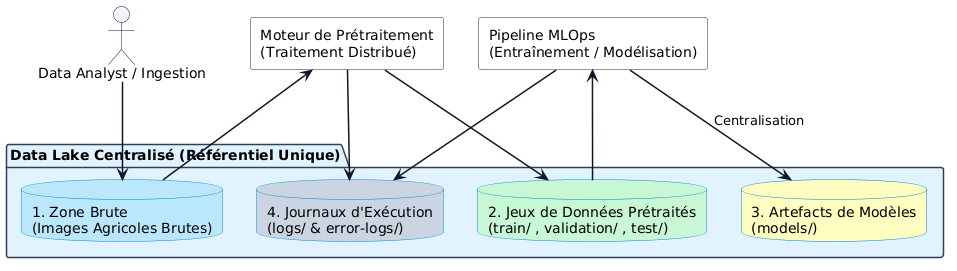
\includegraphics[width=0.9\textwidth]{chapters/chapter03/fig03/Figure_2_1 – Modelisation_fonctionnelle_du_flux_de_donnees_vers_le_Data_Lake.png}
%\rule{0.85\textwidth}{5cm} % Cadre temporaire à effacer quand vous aurez l'image
\caption{Modélisation fonctionnelle du flux de données vers le Data Lake}
\label{fig:besoin_datalake}
\end{figure}

\subsubsection{Pilier 2 : Prétraitement distribué (Ingénierie des données)}
Face à l'incapacité d'une machine unique à traiter les images en un temps raisonnable, le système doit impérativement intégrer un moteur de calcul distribué pour l'équipe Data.

\begin{table}[H]
\centering
\caption{Exigences fonctionnelles liées au prétraitement des images agricoles}
\label{tab:besoins_data_eng}
\renewcommand{\arraystretch}{1.4}
\begin{tabular}{|p{4cm}|p{9.5cm}|}
\hline
\rowcolor{darkgreen!20} \textbf{Fonctionnalité} & \textbf{Description de l'action système} \\ \hline
\textbf{Nettoyage} & Filtrage automatique des images corrompues ou inexploitables avant analyse. \\ \hline
\textbf{Transformation} & Redimensionnement et normalisation des matrices d'images en parallèle. \\ \hline
\textbf{Feature Engineering} & Extraction de caractéristiques visuelles (via Analyse en Composantes Principales - ACP) pour réduire la dimensionnalité des données. \\ \hline
\textbf{Génération de Datasets} & Sauvegarde automatisée des données propres et formatées vers le Data Lake. \\ \hline
\end{tabular}
\end{table}

\subsubsection{Pilier 3 : Environnement de développement et CI/CD}
L'architecture doit faciliter le travail quotidien des équipes techniques (Data Scientists et ingénieurs MLOps) tout en garantissant la reproductibilité du code.
\begin{itemize}
    \item[$\bullet$] \textbf{Espace de travail en libre-service :} Fournir un environnement de développement interactif (Notebooks), directement connecté au Data Lake, sans exiger de configuration d'infrastructure de la part du Data Scientist.
    \item[$\bullet$] \textbf{Automatisation (IaC et CI/CD) :} Le déploiement de l'infrastructure sous-jacente et l'exécution des tests doivent être automatisés via des pipelines d'intégration et de livraison continues déclenchés à chaque modification du code source.
\end{itemize}

% Espace réservé pour votre future image (CI/CD)
\begin{figure}[H]
\centering
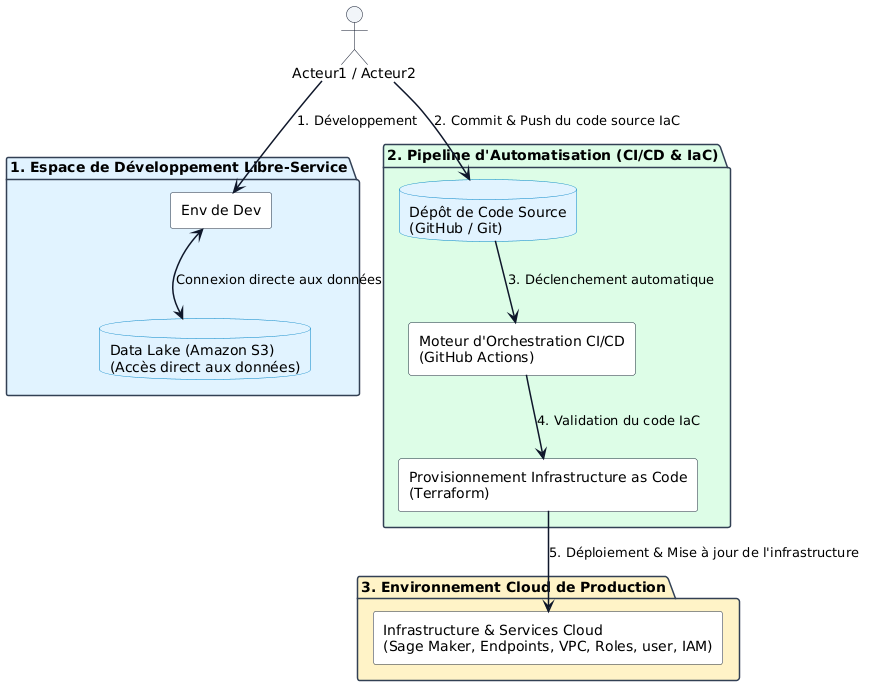
\includegraphics[width=0.85\textwidth]{chapters/chapter03/fig03/image_cicd.png}
%\rule{0.85\textwidth}{4.5cm} % Cadre temporaire à effacer quand vous aurez l'image
\caption{Flux fonctionnel d'Intégration et de Déploiement Continus (CI/CD)}
\label{fig:besoin_cicd}
\end{figure}

\subsubsection{Pilier 4 : Orchestration ML, Registre et Déploiement}
La plateforme doit encadrer le cycle de vie du modèle d'intelligence artificielle de manière reproductible et traçable, en isolant cette étape du traitement de la donnée brute.

\begin{table}[H]
\centering
\caption{Exigences fonctionnelles liées à la Plateforme MLOps}
\label{tab:besoins_mlops}
\renewcommand{\arraystretch}{1.4}
\begin{tabular}{|p{4cm}|p{9.5cm}|}
\hline
\rowcolor{darkgreen!20} \textbf{Fonctionnalité} & \textbf{Description de l'action système} \\ \hline
\textbf{Orchestration (Pipelines)} & Exécution séquentielle et automatisée de l'entraînement du modèle sur les données propres, suivie de son évaluation. \\ \hline
\textbf{Registre de Modèles} & Stockage centralisé et versionnage de chaque modèle entraîné, accompagné de ses métriques de performance et de son lignage. \\ \hline
\textbf{Approbation} & Mécanisme conditionnant le passage d'un modèle candidat vers la production (statut \textit{Approved} ou \textit{Rejected}). \\ \hline
\textbf{Déploiement (Inférence)} & Mise à disposition du modèle validé sous forme de point de terminaison (\textit{Endpoint}) pour réaliser des prédictions sur de nouvelles images. \\ \hline
\end{tabular}
\end{table}

\subsection{Besoins non fonctionnels}
Les besoins non fonctionnels définissent les critères de qualité, de performance et de sécurité auxquels notre architecture Cloud doit impérativement satisfaire. Pour assurer la pérennité du système de vision par ordinateur du client, ces exigences ont été catégorisées en quatre axes majeurs :

\subsubsection{Axe 1 : Scalabilité et Élasticité (Passage à l'échelle)}
Face à la volumétrie massive et imprévisible des images agricoles, l'infrastructure doit être capable de s'adapter dynamiquement à la charge de travail.
\begin{itemize}
    \item[$\bullet$] \textbf{Traitement Big Data :} Le cluster de calcul (\textit{Amazon EMR}) doit pouvoir dimensionner automatiquement ses nœuds de travail (\textit{Worker Nodes}) pour absorber le flux d'images lors d'une campagne de récolte, sans dégradation du temps de traitement.
    \item[$\bullet$] \textbf{Inférence ML :} Les points de terminaison (\textit{Endpoints}) d'\textit{Amazon SageMaker} doivent intégrer des politiques d'élasticité (\textit{Auto Scaling}) pour gérer les pics de requêtes de prédiction en production, tout en maintenant une faible latence.
\end{itemize}

\subsubsection{Axe 2 : Optimisation financière (Approche FinOps)}
Étant donné l'intensité des calculs requis pour le traitement d'images haute résolution et l'extraction de caractéristiques par Analyse en Composantes Principales (ACP), la maîtrise des coûts est une contrainte stricte du cahier des charges.
\begin{itemize}
    \item[$\bullet$] \textbf{Ressources éphémères :} Le cluster de préparation des données (Data Engineering) doit être provisionné à la demande et détruit de manière automatisée dès la fin de la génération des datasets. Il ne doit y avoir aucune facturation de ressources de calcul inactives.
    \item[$\bullet$] \textbf{Instances Spot :} L'architecture doit prioriser l'utilisation de la capacité excédentaire d'AWS (\textit{Instances Spot}) pour les tâches de traitement par lots, permettant de réduire les coûts de calcul de manière significative (jusqu'à 70\% d'économie).
\end{itemize}

\subsubsection{Axe 3 : Sécurité, Isolement et Conformité}
La manipulation de données propriétaires (images de cultures, modèles d'entreprise) nécessite un cloisonnement strict du système, conformément aux bonnes pratiques Cloud.
\begin{itemize}
    \item[$\bullet$] \textbf{Isolation réseau (VPC) :} L'ensemble des ressources (S3, EMR, SageMaker Studio) doit être déployé au sein d'un Réseau Privé Virtuel (\textit{Amazon VPC}), empêchant tout accès direct depuis l'Internet public.
    \item[$\bullet$] \textbf{Gestion des accès (IAM) :} Application stricte du « principe du moindre privilège ». Chaque service AWS (ex: le cluster EMR) et chaque pipeline d'automatisation (\textit{GitHub Actions}) ne doit disposer que des autorisations strictement nécessaires à son exécution.
    \item[$\bullet$] \textbf{Chiffrement :} Toutes les données stockées dans le Data Lake ainsi que les artefacts de modèles doivent être chiffrés au repos et en transit via le service \textit{AWS KMS} (Key Management Service).
\end{itemize}

\subsubsection{Axe 4 : Maintenabilité et Supervision (SRE)}
L'architecture, bien que complexe sous le capot, doit rester observable et facilement maintenable par les équipes techniques.
\begin{itemize}
    \item[$\bullet$] \textbf{Supervision centralisée :} Tous les journaux d'exécution (\textit{logs}) d'EMR et les métriques de performance des modèles SageMaker doivent être centralisés dans \textit{Amazon CloudWatch} pour faciliter le débogage.
    \item[$\bullet$] \textbf{Reproductibilité (IaC) :} Toute modification de l'infrastructure doit pouvoir être reproduite et auditée. L'utilisation de \textit{Terraform} garantit que l'environnement est versionné et auditable comme du code classique.
\end{itemize}

\vspace{0.3cm}
\begin{table}[H]
\centering
\caption{Matrice de synthèse des besoins non fonctionnels de l'architecture}
\label{tab:besoins_non_fonctionnels}
\renewcommand{\arraystretch}{1.4}
\begin{tabular}{|p{3cm}|p{6cm}|p{5cm}|}
\hline
\rowcolor{darkgreen!20} \textbf{Catégorie} & \textbf{Exigence technique} & \textbf{Solutions \& Services AWS} \\ \hline
\textbf{Élasticité} & Redimensionnement automatique selon la charge de données & \textit{Amazon EMR} / \textit{SageMaker Auto Scaling} \\ \hline
\textbf{FinOps} & Utilisation de clusters éphémères et d'instances à coût réduit & Instances \textit{Amazon EC2 Spot} \\ \hline
\textbf{Sécurité} & Chiffrement des données, moindre privilège et isolement réseau & \textit{AWS KMS}, \textit{AWS IAM}, \textit{Amazon VPC} \\ \hline
\textbf{Supervision} & Traçabilité centralisée des métriques et des erreurs & \textit{Amazon CloudWatch} \\ \hline
\textbf{Maintenabilité} & Infrastructure déployable par code, reproductible et versionnée & \textit{Terraform}, \textit{GitHub Actions} \\ \hline
\end{tabular}
\end{table}

\subsection{Acteurs du système}
L'industrialisation d'un modèle de vision par ordinateur via le MLOps est un effort pluridisciplinaire. Le système conçu implique l'interaction de plusieurs acteurs aux profils techniques distincts. Nous les avons répartis en deux grandes catégories : l'équipe Data (qui manipule la donnée et le modèle) et l'équipe Infrastructure (qui gère les ressources Cloud).

\begin{table}[H]
\centering
\caption{Cartographie des acteurs et de leurs responsabilités dans le système}
\label{tab:acteurs_systeme}
\renewcommand{\arraystretch}{1.4}
\begin{tabular}{|p{3.5cm}|p{11cm}|}
\hline
\rowcolor{darkgreen!20} \textbf{Acteur} & \textbf{Rôle et interactions avec le système} \\ \hline
\multicolumn{2}{|c|}{\cellcolor{gray!10}\textbf{Équipe Data}} \\ \hline
\textbf{Data Engineer} \newline (Ingénieur Données) & Responsable de la première partie de l'architecture. Il développe et exécute les scripts de traitement distribué (PySpark) sur le cluster \textit{Amazon EMR}. Il s'assure que les images sont correctement ingérées, nettoyées, transformées (ACP), et sauvegardées de manière structurée dans le Data Lake (\textit{Amazon S3}). \\ \hline
\textbf{Data Scientist} \newline (Scientifique des Données) & Utilisateur principal de la plateforme MLOps. Depuis son environnement \textit{Amazon SageMaker Studio}, il consomme les données propres préparées par le Data Engineer. Il conçoit le code du modèle, lance les tâches d'entraînement (\textit{Training Jobs}) et enregistre les versions candidates du modèle dans le registre (\textit{Model Registry}). \\ \hline
\textbf{Lead Data} \newline (Responsable Data) & Superviseur de la qualité algorithmique. Il analyse les métriques de performance des modèles enregistrés par les Data Scientists. C'est lui qui déclenche manuellement ou valide l'approbation d'un modèle dans le registre, autorisant ainsi son passage vers l'environnement de production. \\ \hline
\multicolumn{2}{|c|}{\cellcolor{gray!10}\textbf{Équipe Infrastructure}} \\ \hline
\textbf{Administrateur Cloud} \newline (Ingénieur MLOps / Cloud) & Garant de la stabilité, de la sécurité et des coûts (FinOps). Il déploie l'infrastructure sous-jacente en tant que code (\textit{Terraform}) via les pipelines CI/CD (\textit{GitHub Actions}). Il configure le réseau (VPC), gère les permissions d'accès (IAM) et supervise l'état des serveurs et les journaux d'erreurs via \textit{Amazon CloudWatch}. \\ \hline
\end{tabular}
\end{table}

\subsection{Diagramme de cas d'utilisation}
La modélisation UML (Unified Modeling Language) permet de cartographier formellement les interactions fonctionnelles entre ces acteurs et le système Cloud. Le diagramme de cas d'utilisation présenté ci-dessous illustre le périmètre de notre architecture hybride, en mettant en évidence la séparation des responsabilités.

Ce diagramme s'articule autour des macro-processus suivants :
\begin{itemize}
    \item[$\bullet$] \textbf{Gestion des données massives :} Ingestion des images brutes et déclenchement du prétraitement distribué (réservé au Data Engineer).
    \item[$\bullet$] \textbf{Cycle de vie du modèle :} Développement, entraînement et enregistrement du modèle (réservé au Data Scientist).
    \item[$\bullet$] \textbf{Gouvernance et Déploiement :} Approbation du modèle (Lead Data) et orchestration de l'infrastructure globale (Administrateur Cloud).
\end{itemize}

% Espace réservé pour votre diagramme UML (Cas d'utilisation)
\begin{figure}[H]
\centering
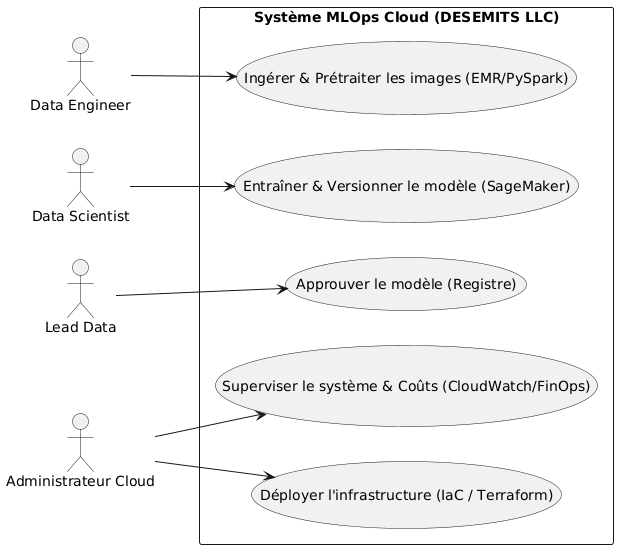
\includegraphics[width=0.9\textwidth]{chapters/chapter02/fig02/dcu.png}
%\rule{0.9\textwidth}{8cm} % Cadre temporaire à effacer quand vous aurez généré votre diagramme UML
\caption{Diagramme de cas d'utilisation du système hybride (Data Engineering \& MLOps)}
\label{fig:usecase_mlops}
\end{figure}


% ==============================================================================
\section{Conception de la solution}
% ==============================================================================

Sur la base de l'analyse des besoins fonctionnels et non fonctionnels, nous avons conçu une architecture Cloud distribuée capable de résoudre les problèmes de saturation locale rencontrés par le client. Le principe fondamental qui dicte cette conception est le \textbf{découplage strict entre le stockage des données et la puissance de calcul}, une bonne pratique incontournable dans l'ingénierie des données massives.

\subsection{Architecture logique}
L'architecture logique modélise le flux de traitement de l'information et l'orchestration des processus, en faisant abstraction des composants matériels ou des serveurs physiques sous-jacents. Ce modèle s'articule autour d'un pipeline divisé en deux grands sous-systèmes interdépendants, conformément à notre positionnement : le sous-système de préparation des données (\textit{Data Engineering}) et le sous-système d'orchestration des modèles (\textit{MLOps}).

Le flux logique de notre système suit un graphe orienté qui se décompose en quatre étapes majeures :

\begin{enumerate}
    \item \textbf{Ingestion et Stockage centralisé :} L'opérateur métier ou le système de collecte dépose un jeu d'images agricoles brutes dans le référentiel central (\textit{Data Lake}). Cet espace agit comme l'unique source de vérité (\textit{Single Source of Truth}) pour l'ensemble du système, isolant les données brutes des données transformées.
    
    \item \textbf{Prétraitement distribué (Pipeline Data) :} Le dépôt des données justifie l'instanciation du moteur de calcul distribué. Ce dernier parallélise les tâches lourdes de préparation : nettoyage des images, redimensionnement, et surtout la réduction de dimensionnalité via une Analyse en Composantes Principales (ACP). Les caractéristiques extraites (\textit{features}) sont re-sauvegardées de manière structurée dans le Data Lake, allégeant ainsi le volume d'information.
    
    \item \textbf{Orchestration et Entraînement (Pipeline ML) :} Une fois les données préparées, le moteur d'orchestration MLOps prend le relais. Il charge les données propres et exécute les scripts d'apprentissage du modèle de vision par ordinateur. Cette étape inclut la validation des performances du modèle candidat sur un jeu de test.
    
    \item \textbf{Gouvernance et Inférence :} Le modèle entraîné est versionné et stocké dans un registre logique (\textit{Model Registry}). Après validation (approbation) par l'équipe Data, il est déployé sur un point de terminaison (\textit{Endpoint}) pour réaliser des prédictions (inférence) sur de nouvelles images. Les résultats prédictifs (détection d'anomalies) sont ensuite sauvegardés dans le Data Lake, clôturant ainsi le cycle logique.
\end{enumerate}

Cette séparation logique garantit que la complexité et la lourdeur du traitement de la donnée brute n'interfèrent pas avec la plateforme de modélisation, assurant ainsi la fluidité et la répétabilité du cycle de vie du modèle.

% Espace réservé pour votre diagramme d'architecture logique
\begin{figure}[H]
\centering
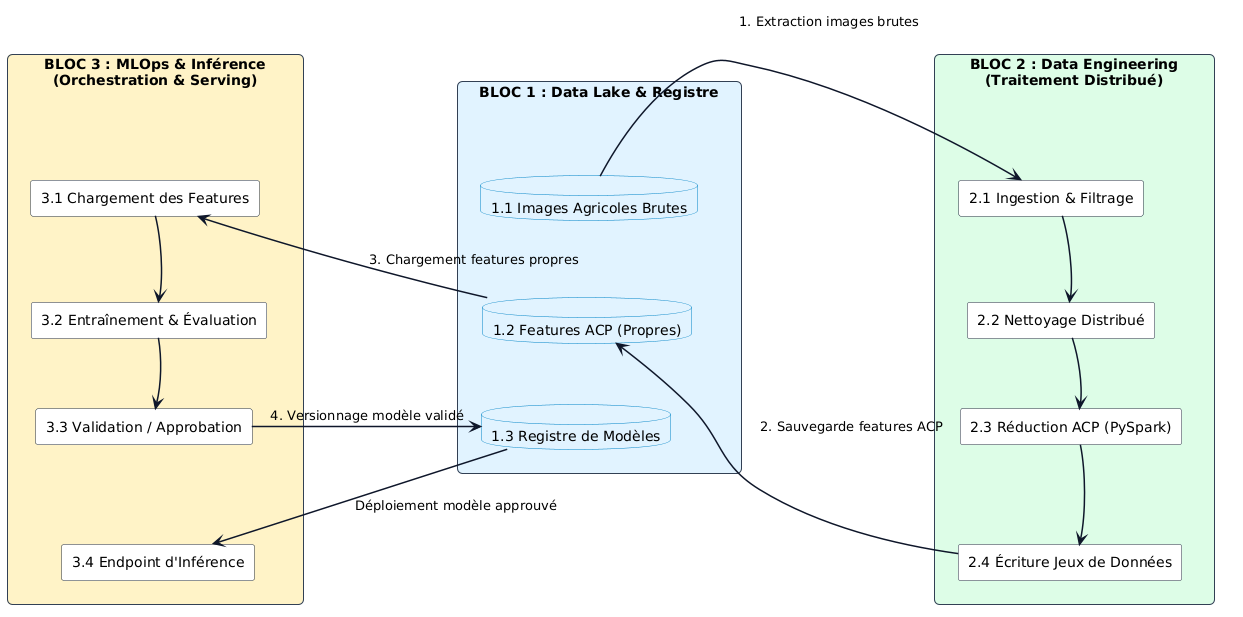
\includegraphics[width=0.9\textwidth]{chapters/chapter03/fig03/2_4_Architecture_logique_du_pipeline_de_traitement.png}
%\rule{0.9\textwidth}{7cm} % Cadre temporaire à effacer quand vous aurez l'image
\caption{Architecture logique du pipeline de traitement distribué et d'orchestration MLOps}
\label{fig:architecture_logique}
\end{figure}

\subsection{Architecture physique}
L'architecture physique matérialise le flux logique décrit précédemment en s'appuyant exclusivement sur les services Cloud managés d'Amazon Web Services (AWS). Conformément à notre positionnement hybride, cette infrastructure déploie des ressources distinctes pour le traitement massif d'un côté, et pour l'orchestration du Machine Learning de l'autre, tout en garantissant un environnement hautement sécurisé.

Les composants physiques de notre architecture se répartissent en quatre couches fonctionnelles :

\subsubsection{Couche 1 : Sécurité et Réseau (Fondations)}
Toute l'architecture repose sur une fondation sécurisée pour protéger les données propriétaires du client :
\begin{itemize}
    \item[$\bullet$] \textbf{Amazon VPC (Virtual Private Cloud) :} L'ensemble des ressources de calcul et des espaces de travail est isolé dans un réseau privé virtuel. Cela permet de contrôler strictement le trafic entrant et sortant via des groupes de sécurité (\textit{Security Groups}) \cite{43}.
    \item[$\bullet$] \textbf{AWS IAM (Identity and Access Management) :} La gouvernance des accès est dictée par des rôles IAM stricts. Par exemple, le cluster EMR ne possède que les droits de lecture/écriture sur le bucket S3 dédié, garantissant l'application du principe de moindre privilège \cite{43}.
\end{itemize}

\subsubsection{Couche 2 : Sous-système Data Engineering (Partie 1)}
Cette couche absorbe la charge lourde du traitement des images agricoles :
\begin{itemize}
    \item[$\bullet$] \textbf{Amazon S3 (Data Lake) :} Service de stockage objet agissant comme le cœur de l'architecture. Il stocke les images brutes, les données transformées (après ACP) et les artefacts des modèles de manière hautement durable et chiffrée.
    \item[$\bullet$] \textbf{Amazon EMR (Elastic MapReduce) :} Le moteur de calcul distribué (utilisant \textit{Apache Spark/PySpark}). Pour respecter nos contraintes FinOps, ce cluster est \textbf{éphémère} : il est instancié avec des instances \textit{Spot} (à coût réduit) uniquement pour la durée de la génération des datasets, puis détruit automatiquement.
\end{itemize}

\subsubsection{Couche 3 : Plateforme MLOps (Partie 2)}
Une fois les jeux de données préparés sur S3, cette couche prend le relais pour le cycle de vie de l'IA :
\begin{itemize}
    \item[$\bullet$] \textbf{Amazon SageMaker Studio :} L'environnement de développement (\textit{IDE}) managé fourni aux Data Scientists. Il permet de développer le code ML dans des Notebooks Jupyter connectés aux données de S3.
    \item[$\bullet$] \textbf{SageMaker Model Registry :} Un registre physique centralisant les versions des modèles entraînés et gérant leur statut d'approbation (ex: \textit{PendingManualApproval} vers \textit{Approved}) \cite{43}.
    \item[$\bullet$] \textbf{SageMaker Endpoints :} L'infrastructure d'inférence. Les modèles validés y sont déployés sous forme d'API REST auto-scalables pour réaliser des prédictions sur de nouvelles images.
\end{itemize}

\subsubsection{Couche 4 : Automatisation et Supervision (CI/CD et IaC)}
Pour relier les composants et assurer la reproductibilité de l'infrastructure :
\begin{itemize}
    \item[$\bullet$] \textbf{Terraform \& GitHub Actions :} L'infrastructure AWS et les pipelines MLOps ne sont pas cliqués manuellement, mais définis sous forme de code (\textit{Infrastructure as Code}). GitHub Actions orchestre le déploiement continu des ressources via Terraform, garantissant que chaque environnement peut être recréé à l'identique.
    \item[$\bullet$] \textbf{Amazon CloudWatch :} Service de supervision qui collecte les métriques d'utilisation (CPU, RAM) des clusters EMR et les journaux d'erreurs des modèles SageMaker pour alerter l'Administrateur Cloud en cas de défaillance.
\end{itemize}

% Espace réservé pour votre diagramme d'architecture physique
\begin{figure}[H]
\centering
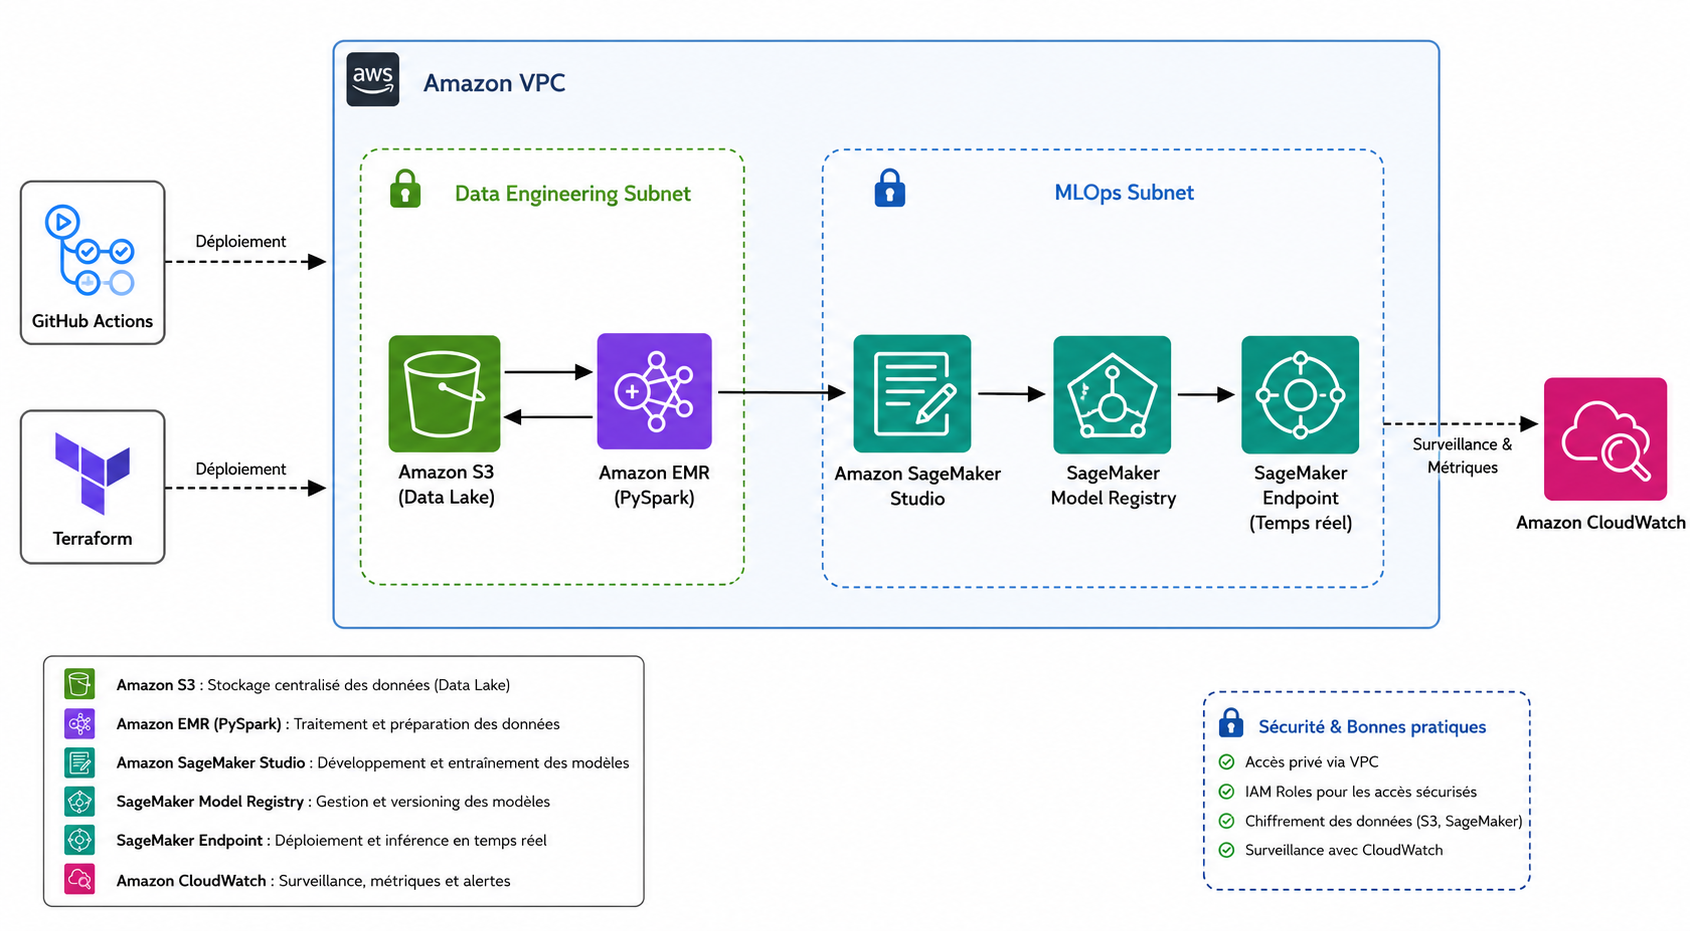
\includegraphics[width=0.95\textwidth]{chapters/chapter03/fig03/2 _5_Architecture_physique.png}
%\rule{0.95\textwidth}{8cm} % Cadre temporaire à effacer quand vous aurez l'image
\caption{Architecture physique détaillée de la solution MLOps sur Amazon Web Services}
\label{fig:architecture_physique}
\end{figure}

% ==============================================================================
\section{Résumé du chapitre}
% ==============================================================================

Ce chapitre a permis de traduire la problématique d'ingénierie soulevée par le client en une solution technique concrète et rigoureusement modélisée. En appliquant une méthodologie de conception itérative basée sur des Sprints, nous avons identifié les limites critiques de l'approche locale initiale et formalisé des besoins stricts en matière de passage à l'échelle, de sécurité et d'optimisation financière (FinOps).

L'analyse des acteurs a clarifié la répartition des tâches au sein de l'organisation : le \textit{Data Engineer} et le \textit{Data Scientist} interagissant avec les données et les modèles, tandis que le \textit{Lead Data} et l'\textit{Administrateur Cloud} assurent la gouvernance et le maintien de l'infrastructure. 

Enfin, la conception architecturale a mis en évidence notre choix stratégique fondamental : un découplage physique via une architecture hybride. Le traitement massif des données est intégralement délégué à un sous-système Big Data éphémère (Amazon EMR et S3), tandis que l'orchestration, le registre et le déploiement du modèle d'intelligence artificielle reposent sur une plateforme MLOps standardisée (Amazon SageMaker, couplé à GitHub et Terraform). 

Ces fondations méthodologiques et architecturales étant désormais solidement établies, le chapitre suivant sera consacré à l'implémentation pratique de cette architecture sur le Cloud AWS et à l'évaluation de ses performances.


% % 🛠️ À FAIRE : Insérer l'Architecture Physique AWS
% \begin{figure}[H]
%     \centering
%     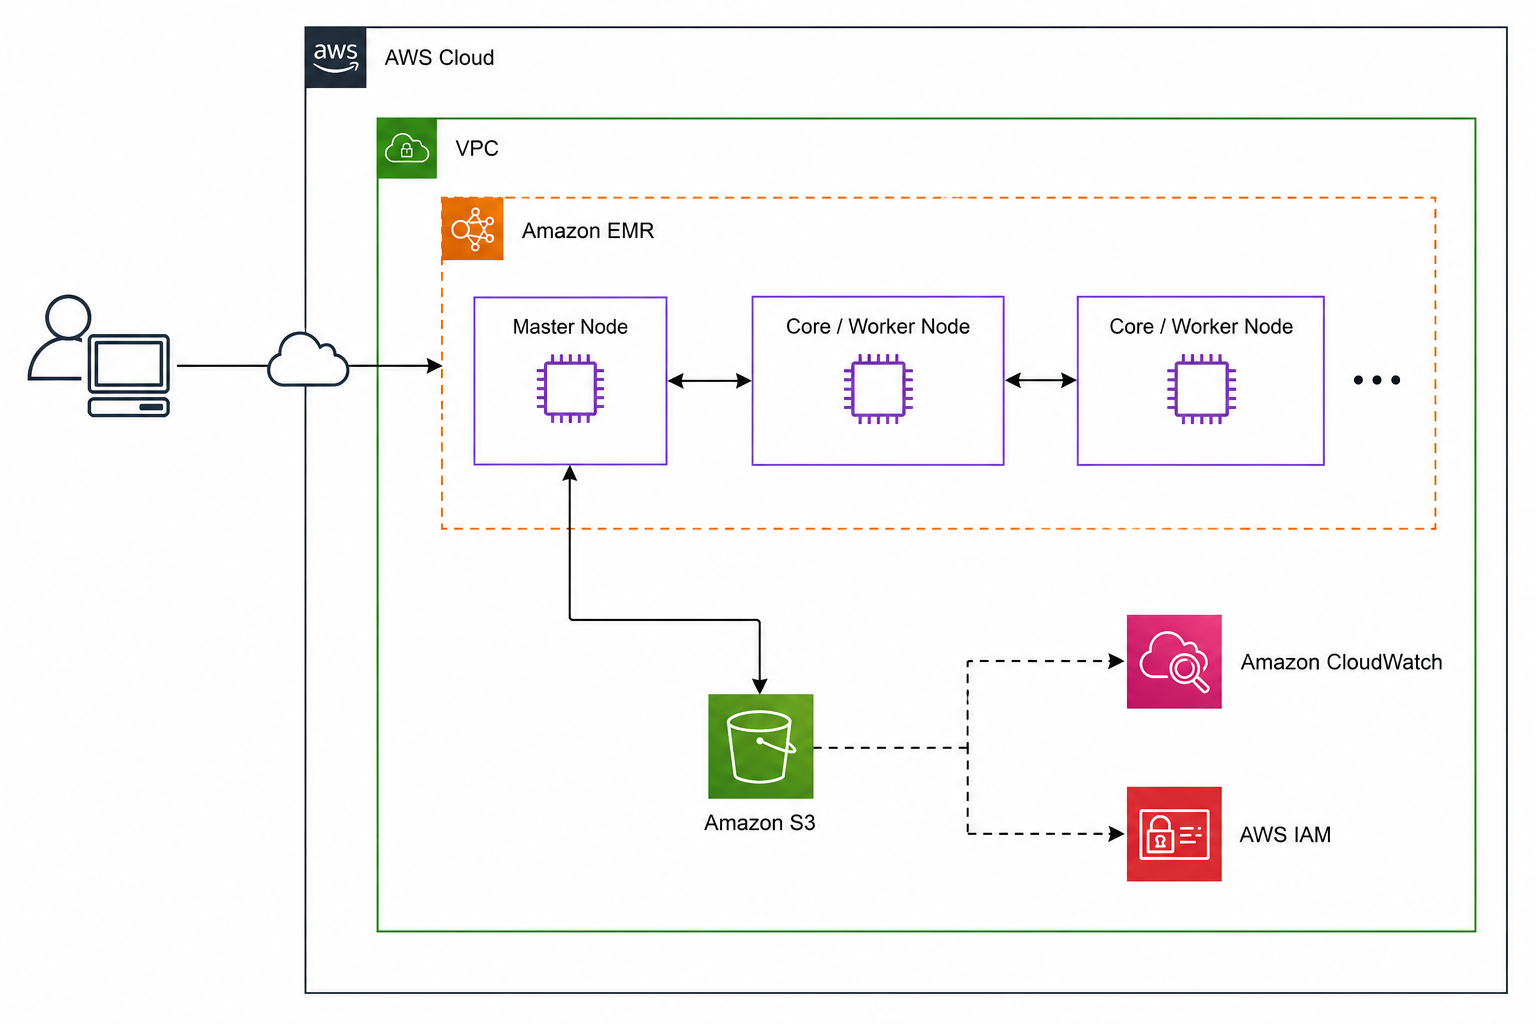
\includegraphics[width=0.9\textwidth]{chapters/chapter03/fig03/2-8-architecture-physique.png}
%     %\rule{0.9\textwidth}{7cm} % Ligne à supprimer quand l'image sera insérée
%     \caption{Architecture physique déployée sur Amazon Web Services}
%     \label{fig:architecture_physique}
% \end{figure}
